\chapter{反应焓}\label{ch:b2:reaction-enthalpy}

一个露营燃气罐拧在小型燃烧器下方：几克丁烷
数分钟内即可把一升水烧开，锅底下的蓝色火焰
远比沸水热。反应放出多少热量，其中有多少
传给锅，火焰又能达到多高温度？这些问题
无需燃烧器即可回答：只需每种物质的几个数值，
测定一次便可一劳永逸，就能给出
可由这些物质写出的每个反应在任意温度下的热量。
本章建立这套核算方法，将物理学中已知的
热力学第一定律用于组成会变化的系统，
把反应焓定义为偏导数，
并由生成焓、键焓以及沿循环途径进行计算，
说明它如何随温度变化，
以及它与火焰和量热计的关系。

\begin{recall}
物理学中已知：热力学第一定律 $\Delta U = W + Q$；焓 $H = U + pV$，
为状态函数；在恒定外压下，于该压强下的两个状态之间，
吸收的热量为 $Q_p = \Delta H$；定压热容
$C_p = (\partial H/\partial T)_p$；理想气体的焓仅依赖于 $T$。
本科一年级分册描述了反应体系，
以反应进度 $\xi$ 和化学计量数 $\nu_i$ 刻画其组成，
其中 $0 = \sum_i\nu_i\mathrm A_i$ 为反应式，并规定每种物种
的标准态为 $p^\circ = \qty{1}{bar}$。第 1 册（十一年级）称放出热量的
反应为放热反应，并利用键能
估算燃烧能。
\end{recall}

\begin{omfigure}
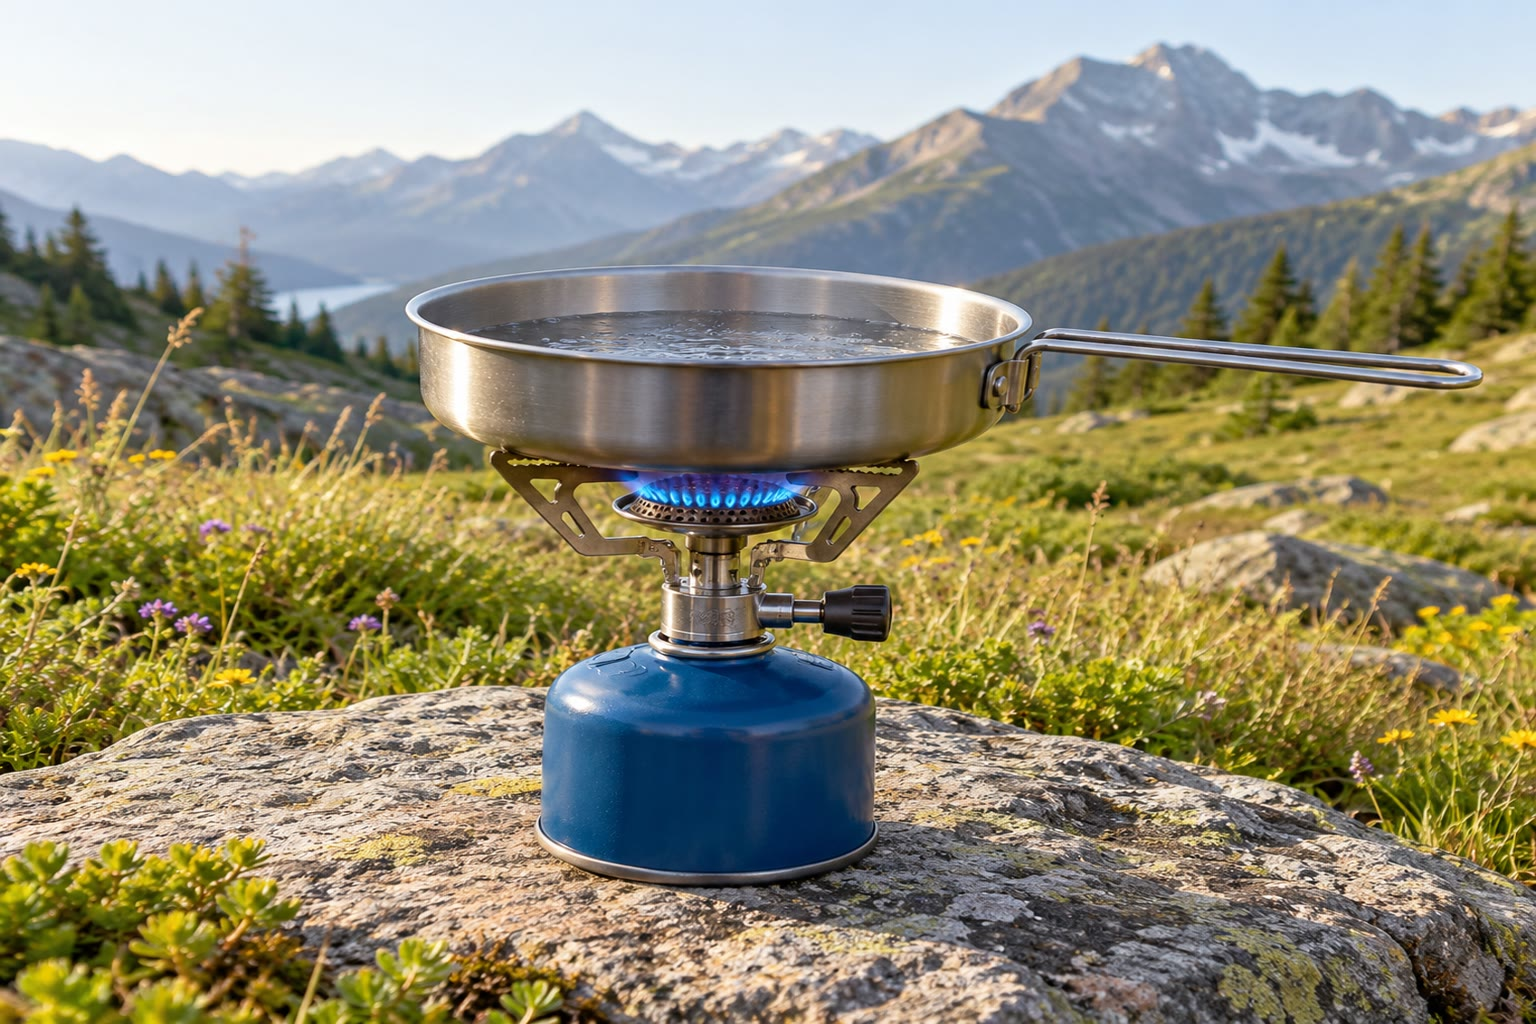
\includegraphics[width=0.6\linewidth]{images/book3/ai/b2-01-camping-stove.jpg}

{\small 露营炉：燃气罐中的丁烷在锅下方的空气中燃烧，
每摩尔丁烷释放的热量、传给水的热量份额
以及火焰温度，均在本章的
周末问题中计算。}
\end{omfigure}

\section{反应量}

在发生单一反应 $0 = \sum_i\nu_i\mathrm A_i$ 的封闭系统中，
该系统由其温度、压强和反应进度描述：
各物质的量为 $n_i = n_{i,0} + \nu_i\xi$。系统的每个广延状态函数，
例如焓，则是 $H(T, p,
\xi)$ 的函数，其全微分为
\[
  \dd H = \left(\frac{\partial H}{\partial T}\right)_{p,\xi}\dd T
        + \left(\frac{\partial H}{\partial p}\right)_{T,\xi}\dd p
        + \left(\frac{\partial H}{\partial \xi}\right)_{T,p}\dd\xi .
\]

\begin{definition}[反应量、反应焓]\label{def:b2:reaction-enthalpy:reaction-quantity}
对于封闭系统的广延状态函数 $X$，该系统中发生
反应 $0 = \sum_i\nu_i\mathrm A_i$ 时，\emph{反应
量}\index{反应量}为偏导数
\[
  \Delta_r X = \left(\frac{\partial X}{\partial \xi}\right)_{T,p} ,
\]
即在定温定压下，单位反应进度引起的 $X$ 的变化，
以每摩尔 $X$ 单位计。对 $X = H$，它就是\emph{反应
焓}\index{反应焓} $\Delta_r H$，单位为 \unit{kJ/mol}。
\end{definition}

\begin{remark}[导数，而非差值]\label{rem:b2:reaction-enthalpy:operator}
符号 $\Delta_r$ 是一个算符，作用于体系的状态，
但不改变该状态。改写反应的方式
（系数加倍）使 $\Delta_r H$ 加倍，因此反应量
离开其方程式便无意义。当使用物种的偏摩尔焓
$\bar H_i = (\partial H/\partial n_i)_{T,p,n_j}$ 时，
（见\cref{ch:b2:chemical-potential}），$\Delta_r H = \sum_i\nu_i\bar H_i$，
由 $n_i = n_{i,0} + \nu_i\xi$ 的链式法则得出。
\end{remark}

\begin{proposition}[定温定压下吸收的热量]\label{prop:b2:reaction-enthalpy:qp}
若反应进度在系统中由 $\xi_1$ 推进到 $\xi_2$，
而系统保持 $T$ 和 $p$ 恒定，则系统吸收的热量为
\[
  Q_p = \int_{\xi_1}^{\xi_2}\Delta_r H\,\dd\xi = \Delta_r H\,(\xi_2 - \xi_1)
\]
当 $\Delta_r H$ 不依赖于 $\xi$ 时。
\end{proposition}

\begin{proof}
在恒定 $p$（此处外压亦恒定）下，吸收的热量
即焓变 $Q_p = \Delta H$（物理学结论）。在 $T$ 和 $p$ 固定时，
$H$ 的微分化为 $\dd H = \Delta_r H\,\dd\xi$；积分
从 $\xi_1$ 到 $\xi_2$ 即得结论。
\end{proof}

\begin{definition}[放热的、吸热的、无热效应的]\label{def:b2:reaction-enthalpy:exothermic}
在给定状态下，若反应为\emph{放热的}\index{放热的}，
即 $\Delta_r H < 0$：在恒定 $T$ 和 $p$ 下正向进行时，
它向外界放热。若为\emph{吸热的}\index{吸热的}，则 $\Delta_r H >
0$；若为\emph{无热效应的}\index{无热效应的}，则 $\Delta_r H = 0$。
\end{definition}

一般而言，反应热不依赖于组成：
对于理想气体及纯固体和纯液体，每种物质的焓
与其周围环境无关，$\Delta_r H$ 在
$T$ 确定后即随之确定。

\begin{proposition}[理想系统]\label{prop:b2:reaction-enthalpy:ideal}
在理想气体混合物与纯凝聚相组成的体系中，$\Delta_r H$
仅依赖于温度，且等于
下文定义的标准反应焓 $\Delta_r H^\circ(T)$。对于稀
溶液中的溶质，该等式在较好近似下成立。
\end{proposition}

\begin{proof}
在理想气体混合物中，每种气体的行为如同单独存在，其焓
$n_iH_{m,i}(T)$ 不依赖于 $p$（物理学结论：理想气体的焓
仅依赖于 $T$）。纯固体或纯液体有 $H = n_iH_{m,i}(T,
p)$，且 $(\partial H_m/\partial p)_T = V_m(1 - \alpha T)$ 约为
几 \unit{J/(mol.bar)}，对凝聚相而言与反应焓相比可忽略，
而反应焓为数十 \unit{kJ/mol}。故 $H = \sum_in_iH_{m,i}(T)$，其
对 $\xi$ 的导数为 $\sum_i\nu_iH_{m,i}(T)$，它仅依赖于
$T$ 而定，其值即所有物种均处于
标准态时算得的值。
\end{proof}

\section{标准反应焓与盖斯定律}

\begin{definition}[标准反应量]\label{def:b2:reaction-enthalpy:standard-reaction-enthalpy}
称\emph{标准反应量}\index{标准反应量}
$\Delta_r X^\circ(T) = \sum_i\nu_iX_{m,i}^\circ(T)$ 为各物种均处于标准态、温度为 $T$ 时算得的反应量，
其中 $X_{m,i}^\circ$ 为标准摩尔量，
对 $X = H$，它即为
\emph{标准反应焓}\index{标准反应焓}
$\Delta_r H^\circ(T)$；它只依赖于 $T$。
\end{definition}

只有焓差可以测量，因此需要选定一个参考点，
并一劳永逸地确定，正如为电势选定氢电极那样。

\begin{definition}[标准参考态、标准摩尔生成焓]\label{def:b2:reaction-enthalpy:formation}
称\emph{标准参考态}\index{标准参考态}为元素在温度 $T$ 下的
最稳定的形态，其温度为 $T$、压强为 $p^\circ$：
\ce{H2}、\ce{O2}、\ce{N2} 和 \ce{Cl2} 取理想气体形式，碳取
石墨形式，钠取金属形式，溴取液体形式（温度为 \qty{298}{K}）。
称\emph{标准摩尔生成焓}\index{标准摩尔生成焓}
$\Delta_f H^\circ$ 为化合物生成反应的标准反应焓，
即由参考态的元素生成一摩尔该
化合物的那个反应。由构造可知，
$\Delta_f H^\circ = 0$ 对处于参考态的元素成立。
\end{definition}

\begin{example}[生成反应]\label{ex:b2:reaction-enthalpy:formation}
水的生成反应为 \ce{H2(g) + 1/2O2(g) -> H2O(l)}，
$\Delta_f H^\circ = \qty{-285.83}{kJ/mol}$（\qty{298.15}{K}）；
甲烷的生成反应为 \ce{C(s) + 2H2(g) -> CH4(g)}，$\Delta_f H^\circ =
\qty{-74.9}{kJ/mol}$；一氧化氮的生成反应为 \ce{1/2N2(g) + 1/2O2(g) ->
NO(g)}，$\Delta_f H^\circ = \qty{+90.3}{kJ/mol}$：一种吸热化合物，
但发动机的热燃气仍会生成它。半整数系数
并不构成问题：生成反应只是一种记账工具，而非
反应机理。
% ledger: dfh:H2O-l, dfh:CH4_g, dfh:NO_g
\end{example}

\begin{theorem}[盖斯定律]\label{thm:b2:reaction-enthalpy:hess}
若某反应是系数分别为 $\lambda_k$ 的若干反应 $k$ 之和，
则其标准反应焓即为这些反应的标准反应焓以相同系数组合的结果：
$\Delta_r H^\circ = \sum_k\lambda_k\Delta_r H_k^\circ$
（\emph{盖斯定律}\index{盖斯定律}）。特别地，标准反应焓
可沿任何由反应物通向
生成物的反应路径来计算。
\end{theorem}

\begin{proof}
每个 $\Delta_r H_k^\circ = \sum_i\nu_{i,k}H_{m,i}^\circ$ 都
对化学计量数呈线性。若反应为 $\sum_k\lambda_k$ 倍的
反应 $k$，则其化学计量数为 $\nu_i = \sum_k\lambda_k
\nu_{i,k}$，于是 $\Delta_r H^\circ = \sum_i\nu_iH_{m,i}^\circ = \sum_k\lambda_k
\sum_i\nu_{i,k}H_{m,i}^\circ$。其背后的依据是热力学第一定律：$H$ 是一个
状态函数，因此在相同始末态之间，其变化量
与路径无关。
\end{proof}

\begin{proposition}[由生成焓求反应焓]\label{prop:b2:reaction-enthalpy:formation-sum}
$\Delta_r H^\circ(T) = \sum_i\nu_i\,\Delta_f H_i^\circ(T)$.
\end{proposition}

\begin{proof}
取如下路径：先将反应物分解为其参考态下的元素
（即其生成反应的逆反应，
系数为 $-\nu_i > 0$），然后由相同元素生成产物
（系数为 $\nu_i > 0$）。因方程已配平，元素相消，
再由盖斯定律将各焓值相加。
\end{proof}

\begin{omfigure}
\begin{tikzpicture}[font=\small, >={Stealth}, y=0.0062cm]
  \draw[->] (0,-1000) -- (0,180) node[above] {$H^\circ$ (\unit{kJ/mol})};
  \foreach \y in {0,-200,-400,-600,-800,-1000} \draw (-0.08,\y) -- (0.08,\y) node[left=4pt] {$\y$};
  % levels
  \draw[very thick] (1.0,0) -- (4.6,0) node[right] {\ce{C(s) + 2H2(g) + 2O2(g)}};
  \draw[very thick, omDef] (1.0,-74.9) -- (4.6,-74.9);
  \node[right, omDef] at (4.6,-110) {\ce{CH4(g) + 2O2(g)}};
  \draw[very thick, omThm] (1.0,-965.2) -- (4.6,-965.2) node[right] {\ce{CO2(g) + 2H2O(l)}};
  % arrows
  \draw[->, omDef, thick] (1.6,0) -- (1.6,-74.9);
  \node[omDef, anchor=south west, font=\footnotesize] at (1.1,5) {$\Delta_f H^\circ(\ce{CH4}) = -74.9$};
  \draw[->, omThm, thick] (3.9,0) -- (3.9,-965.2);
  \node[right, omThm, align=left] at (3.95,-500) {$\Delta_f H^\circ(\ce{CO2})$\\ $+ 2\Delta_f H^\circ(\ce{H2O})$\\ $= -965.2$};
  \draw[->, thick] (2.75,-74.9) -- (2.75,-965.2);
  \node[left, align=right] at (2.7,-650) {$\Delta_r H^\circ$\\ $= -890.3$};
\end{tikzpicture}

{\small 甲烷燃烧在 \qty{298.15}{K} 时的焓能级。
处于参考态的元素取作零点。甲烷位于
它们之下 \qty{74.9}{kJ/mol}，生成物则在 \qty{965.2}{kJ/mol} 之下：
燃烧焓即两者之差 \qty{-890.3}{kJ/mol}，无论
火焰实际经由何种路径。}
% ledger: dfh:CH4_g, dfh:CO2, dfh:H2O-l
\end{omfigure}

\begin{example}[甲烷的燃烧]\label{ex:b2:reaction-enthalpy:methane}
对于 \ce{CH4(g) + 2O2(g) -> CO2(g) + 2H2O(l)}，
$\Delta_r H^\circ = -393.51 + 2(-285.83) - (-74.87) - 0 =
\qty{-890.3}{kJ/mol}$（\qty{298.15}{K}）。量热计中测得的
值为 \qty{-890.7}{kJ/mol}：表中数据与火焰所得结果
在数据的不确定度范围内相符。若水以蒸气形式
离开（$\Delta_f H^\circ = \qty{-241.83}{kJ/mol}$），$\Delta_r H^\circ =
\qty{-802.3}{kJ/mol}$：二者之差 \qty{88.0}{kJ} 即为两摩尔水的
汽化焓，燃气锅炉通过
使烟气凝结而将其回收。
% ledger: dfh:CO2, dfh:H2O-l, dfh:CH4_g, dch:CH4, dfh:H2O_g (computed in figdata/bachelor-2/thermo-data.py)
\end{example}

\begin{method}[盖斯循环]\label{met:b2:reaction-enthalpy:hess-cycle}
求无法直接测量的反应的焓：
\begin{enumerate}
  \item 写出目标反应及各物种的状态；
  \item 找出焓值已知的反应（如燃烧反应、生成反应），
        其线性组合（系数为 $\lambda_k$）给出目标反应；
  \item 检查所有不在目标反应中出现的物种是否都能相消；
  \item 以相同系数将各焓值相加。
\end{enumerate}
\end{method}

\begin{example}[碳生成一氧化碳]\label{ex:b2:reaction-enthalpy:co}
燃烧碳时总会生成一些二氧化碳，因此
\ce{C(s) + 1/2O2(g) -> CO(g)} 的焓无法直接测量。两个燃烧反应
\ce{C(s) + O2(g) -> CO2(g)}（$\qty{-393.51}{kJ/mol}$）与 \ce{CO(g) +
1/2O2(g) -> CO2(g)}（$\qty{-283.0}{kJ/mol}$，可测得）的焓是已知的；目标反应为
前者减去后者：$\Delta_r H^\circ = -393.51 + 283.0 =
\qty{-110.5}{kJ/mol}$，即一氧化碳的生成焓。
% ledger: dfh:CO2, dfh:CO_g
\end{example}

\begin{history}[日尔曼·昂利·盖斯]
\begin{minipage}[t]{0.2\linewidth}\vspace{0pt}
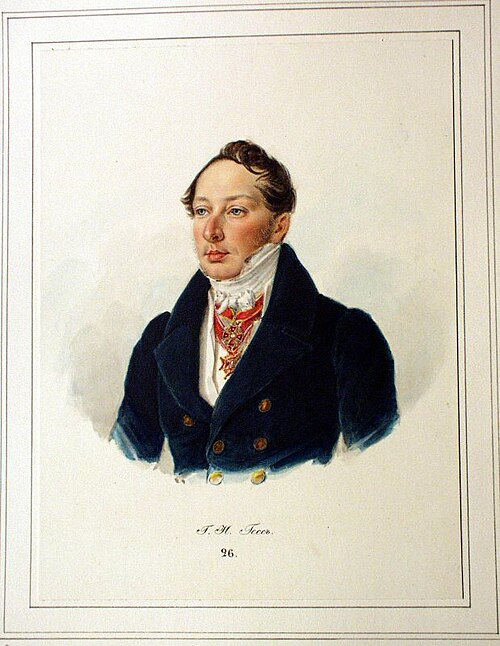
\includegraphics[width=\linewidth]{images/book3/hess.jpg}
\end{minipage}\hfill
\begin{minipage}[t]{0.76\linewidth}\vspace{0pt}
日尔曼·昂利·盖斯（1802--1850）曾任圣彼得堡大学化学教授，
测量了硫酸在分步稀释或中和过程中放出的热量，
于 1840 年发现总热量与所经历的步骤无关，
即“热量总和恒定定律”，该定律先于热力学第一定律提出，
而后者正是对它的解释。
（肖像：I. I. 赖默斯，1837--1838；CC BY-SA 4.0，维基共享资源。）
\end{minipage}
\end{history}

\section{反应焓的计算}

\subsection*{由键焓计算}

当某化合物的生成焓缺失时，
可借助其化学键的能量，在气相中作出估算。

\begin{definition}[键解离焓，平均键焓]\label{def:b2:reaction-enthalpy:bond-enthalpy}
气态分子中某一键 A--B 的\emph{键解离焓}\index{键解离焓}，
是该键断裂为两个气态片段的标准反应焓，
即 \ce{AB(g) -> A(g) + B(g)}，
对双原子分子而言。若分子含 $n$ 个相同的键，其
\emph{平均键焓}\index{平均键焓}为
该分子完全原子化为气态原子的标准焓除以 $n$。
\end{definition}

原子化焓本身即是生成焓：
等于气态原子的生成焓之和，减去分子的生成焓。
下表即按此方法计算。

\begin{omfigure}
\begin{tabular}{lrl}
\hline
键 & 键焓 (\unit{kJ/mol}) & 数据来源 \\
\hline
H--H & 436 & \ce{H2}，解离 \\
O=O & 498 & \ce{O2}，解离 \\
N$\equiv$N & 945 & \ce{N2}，解离 \\
Cl--Cl & 243 & \ce{Cl2}，解离 \\
H--Cl & 432 & \ce{HCl}，解离 \\
C--H & 416 & \ce{CH4}，四个键的平均值 \\
N--H & 391 & \ce{NH3}，三个键的平均值 \\
O--H & 464 & \ce{H2O}，两个键的平均值 \\
C=O & 804 & \ce{CO2}，两个键的平均值 \\
C--C & 330 & \ce{C2H6}，C--H 键取自甲烷 \\
C=C & 589 & \ce{C2H4}，C--H 键取自甲烷 \\
\hline
\end{tabular}

\smallskip
{\small 键焓为 \qty{298.15}{K} 时的数值，由气态原子及分子的标准
生成焓算得。表末两行显示了该方法的局限：
乙烷中的 C--H 键并不完全等同于甲烷中的
C--H 键，因此 C--C 键焓的数值也受其影响。}
% ledger: dfh:C_g, janaf:H, dfh:O_g, dfh:N_g, janaf:Cl, janaf:HCl, dfh:CH4_g, dfh:NH3_g, dfh:H2O_g, dfh:CO2, dfh:C2H6_g, dfh:C2H4_g (computed in figdata/bachelor-2/thermo-data.py)
\end{omfigure}

\begin{proposition}[由键焓估算]\label{prop:b2:reaction-enthalpy:bond-estimate}
对于气相反应，
\[
  \Delta_r H^\circ \approx \sum(\text{断裂键的焓}) -
  \sum(\text{形成键的焓}).
\]
\end{proposition}

\begin{proof}
沿着将每个反应物原子化的路径（焓：断裂键之和），
再由原子组成各生成物（减去形成键的焓）。由盖斯
定律可知，当每个键焓都取自该键所在分子本身时，该和式严格成立；
若以另一分子中的平均值代替，
则为近似。
\end{proof}

\begin{example}[乙烯加氢]\label{ex:b2:reaction-enthalpy:hydrogenation}
在 \ce{C2H4(g) + H2(g) -> C2H6(g)} 中，断裂一个 C=C 键与一个 H--H 键，
生成一个 C--C 键与两个 C--H 键。由表计算：$589 + 436 - 330 - 2
\times 416 = \qty{-137}{kJ/mol}$；由生成焓计算，结果为
\qty{-136.3}{kJ/mol}。此处吻合良好，因为表中的 C--C
键与 C=C 键正是由这些分子得到的；对于
与表中分子不同的分子，误差达 10 至 \qty{30}{kJ/mol} 是常见的。
% ledger: dfh:C2H4_g, dfh:C2H6_g
\end{example}

\subsection*{晶格焓：玻恩–哈伯循环}

\begin{definition}[晶格焓]\label{def:b2:reaction-enthalpy:lattice-enthalpy}
离子晶体的\emph{晶格焓}\index{晶格焓}，
是其解离为气态离子时的标准反应焓：
以氯化钠为例，即 \ce{NaCl(s) -> Na+(g) + Cl-(g)}。晶格焓为正值，
它衡量晶体的内聚强度。
\end{definition}

晶格焓无法直接测量，但可通过经由各元素的循环，
由可测量的量求得：晶体的生成焓、
各元素的原子化焓、金属的电离能与
非金属的电子亲和能（二者均在本科一年级分册中定义）。

\begin{omfigure}
\begin{tikzpicture}[font=\small, >={Stealth}, y=0.0058cm]
  \def\lw{5.0}
  % levels (kJ/mol relative to Na(s) + 1/2 Cl2(g))
  \draw[thick] (0,0) -- (\lw,0) node[right] {\ce{Na(s) + 1/2Cl2(g)}};
  \draw[thick] (0,107.5) -- (\lw,107.5) node[right] {\ce{Na(g) + 1/2Cl2(g)}};
  \draw[thick] (0,228.8) -- (\lw,228.8) node[right] {\ce{Na(g) + Cl(g)}};
  \draw[thick] (0,724.6) -- (\lw,724.6) node[right] {\ce{Na+(g) + e- + Cl(g)}};
  \draw[thick] (0,376.1) -- (\lw,376.1) node[right] {\ce{Na+(g) + Cl-(g)}};
  \draw[thick] (0,-411.1) -- (\lw,-411.1) node[right] {氯化钠 \ce{NaCl(s)}};
  % the path through the elements, on the left
  \draw[->, omDef] (0.4,0) -- (0.4,107.5);
  \node[omDef, left, font=\footnotesize] at (0.35,53) {升华 $107.5$};
  \draw[->, omDef] (0.4,107.5) -- (0.4,228.8);
  \node[omDef, left, font=\footnotesize] at (0.35,168) {$\tfrac12$ 解离 $121.3$};
  \draw[->, omDef] (0.4,228.8) -- (0.4,724.6);
  \node[omDef, left, font=\footnotesize] at (0.35,480) {钠的电离 $495.8$};
  \draw[->, omThm] (1.4,724.6) -- (1.4,376.1);
  \node[omThm, right, font=\footnotesize] at (1.45,560) {电子附着 $-348.6$};
  \draw[->, omProp] (2.3,0) -- (2.3,-411.1);
  \node[omProp, left, font=\footnotesize] at (2.25,-205) {生成焓 $-411.1$};
  % the lattice enthalpy, the only unknown
  \draw[->, thick] (3.6,-411.1) -- (3.6,376.1);
  \node[right, font=\footnotesize] at (3.65,-205) {晶格焓 $787$};
\end{tikzpicture}

{\small 氯化钠在 \qty{298}{K} 时的玻恩–哈伯循环
（\unit{kJ/mol}）。由晶体沿晶格焓上升至气态离子，
或经单质绕行，都到达同一能级：
晶格焓是该循环中唯一的未知量。}
% ledger: dfh:NaCl_cr, dfh:Na_g, janaf:Cl, ie:Na, ea:Cl
\end{omfigure}

\begin{method}[玻恩–哈伯循环]\label{met:b2:reaction-enthalpy:born-haber}
\begin{enumerate}
  \item 从处于参考态的单质出发，画两条路径：一条
        通向晶体（生成），另一条通向气态离子（金属
        的升华、非金属的原子化、电离、电子
        附着）。
  \item 以晶格焓闭合循环，由晶体上升至
        气态离子。
  \item 写出循环中各焓变之和为零，
        并解出未知量。电离能与电子亲和能
        以每个原子的 eV 值列表给出，需乘以 $N_A e = \qty{96.485}{kJ/(mol.eV)}$。
\end{enumerate}
\end{method}

\begin{example}[氯化钠]\label{ex:b2:reaction-enthalpy:nacl}
$\Delta_{\text{晶格}}H^\circ = 411.1 + 107.5 + 121.3 + 495.8 - 348.6 =
\qty{787}{kJ/mol}$。电离能与电子亲和能
均为 \qty{0}{K} 时的能量；修正到 \qty{298}{K} 的修正项（各为 $+\tfrac52RT$，
每项）在两步间相互抵消。点电荷晶体模型
给出相近的数值，这正是氯化钠被称为离子晶体的原因。
% ledger: dfh:NaCl_cr, dfh:Na_g, janaf:Cl, ie:Na, ea:Cl (computed in figdata/bachelor-2/thermo-data.py)
\end{example}

\section{反应焓与温度}

表中给出 $\Delta_f H^\circ$ 在 \qty{298.15}{K} 时的值。反应器的
运行温度为 \qty{700}{K}，火焰则为 \qty{2000}{K}：$\Delta_r H^\circ$ 如何随
温度变化？

\begin{theorem}[基尔霍夫定律]\label{thm:b2:reaction-enthalpy:kirchhoff}
\[
  \frac{\dd\Delta_r H^\circ}{\dd T} = \Delta_r C_p^\circ =
  \sum_i\nu_i C_{p,m,i}^\circ ,
\]
于是 $\Delta_r H^\circ(T_2) = \Delta_r H^\circ(T_1) + \int_{T_1}^{T_2}
\Delta_r C_p^\circ\,\dd T$（\emph{基尔霍夫定律}\index{基尔霍夫定律}），
在 $T_1$ 与 $T_2$ 之间无相变时成立。
\end{theorem}

\begin{proof}
各物种均处于标准态时，$H^\circ(T, \xi) = \sum_in_i
H^\circ_{m,i}(T)$ 是两个变量的函数，其二阶偏导数
连续；由施瓦茨定理，二者可交换：
\[
  \frac{\dd\Delta_r H^\circ}{\dd T} = \frac{\partial}{\partial T}
  \frac{\partial H^\circ}{\partial\xi} = \frac{\partial}{\partial\xi}
  \frac{\partial H^\circ}{\partial T} = \frac{\partial}{\partial\xi}
  \sum_in_iC^\circ_{p,m,i} = \sum_i\nu_iC^\circ_{p,m,i}.
\]
对 $T_1$ 到 $T_2$ 积分即得第二式。若区间内
某物种发生相变，则需计入其相变焓，
并乘以化学计量数。
\end{proof}

\begin{example}[高温下的合成氨]\label{ex:b2:reaction-enthalpy:kirchhoff}
对于 \ce{N2(g) + 3H2(g) -> 2NH3(g)}，$\Delta_r H^\circ(298) =
\qty{-91.9}{kJ/mol}$，取 \qty{298}{K} 时的热容，
$\Delta_r C_p^\circ = 2(35.65) - 29.12 - 3(28.84) =
\qty{-44.3}{J/(K.mol)}$。若视为常数，则得 $\Delta_r
H^\circ(700) = -91.9 - 0.0443 \times 402 = \qty{-109.7}{kJ/mol}$。表中
数据考虑了热容随温度的增大，给出
\qty{-105.2}{kJ/mol}。恒定 $C_p$ 的估算偏差为 4\,\%，
一步计算的合理代价。超过 \qty{400}{K} 时，反应
焓约变化七分之一。
% ledger: dfh:NH3_g, cp:NH3_g.298, cp:N2_g.298, cp:H2_g.298, janafdfH:NH3.700 (computed in figdata/bachelor-2/thermo-data.py)
\end{example}

\section{绝热反应与量热法}

\subsection*{火焰温度}

火焰中反应很快，热量来不及散出：
气体自身被加热。

\begin{definition}[绝热火焰温度]\label{def:b2:reaction-enthalpy:flame-temperature}
燃料的\emph{绝热火焰温度}\index{绝热火焰温度}，是指
其完全燃烧产物所达到的温度，
即在恒压、无任何热量交换的条件下进行反应，
且反应物初始温度为 \qty{298}{K}。
\end{definition}

\begin{proposition}[计算火焰温度]\label{prop:b2:reaction-enthalpy:flame}
若反应进行了 $\xi$ 的反应进度（反应物温度为 $T_0$），且终态
体系的热容为 $C_p(T)$，则终温 $T_f$ 满足
\[
  \xi\,\Delta_r H^\circ(T_0) + \int_{T_0}^{T_f}C_p(T)\,\dd T = 0 .
\]
\end{proposition}

\begin{proof}
绝热且恒压，过程有 $\Delta H =
Q_p = 0$。$H$ 是状态函数，因此在相同的始态与
终态之间，任意路径给出的 $\Delta H$ 相同。取下图所示的路径：
先在 $T_0$ 下进行反应，
$\Delta H_1 = \xi\Delta_r H^\circ(T_0)$（\cref{prop:b2:reaction-enthalpy:qp}，
取理想行为）；再将终态体系从 $T_0$ 加热到
$T_f$，$\Delta H_2 = \int C_p\,\dd T$。二者之和为零。
\end{proof}

\begin{omfigure}
\begin{tikzpicture}[font=\small, >={Stealth}]
  \draw[->] (0,0) -- (6.2,0) node[right] {反应进度 $\xi$};
  \draw[->] (0,0) -- (0,3.6) node[above] {温度 $T$};
  \fill (0.6,0.6) circle (2pt) node[below left] {反应物，$T_0$};
  \fill (5.2,0.6) circle (2pt) node[below] {生成物，$T_0$};
  \fill (5.2,3.0) circle (2pt) node[right] {生成物，$T_f$};
  \draw[->, thick, omDef] (0.7,0.6) -- (5.1,0.6);
  \node[omDef, above, font=\footnotesize] at (3.15,0.64) {$\Delta H_1 = \xi\,\Delta_r H^\circ(T_0) < 0$};
  \draw[->, thick, omThm] (5.2,0.7) -- (5.2,2.9);
  \node[omThm, right, align=left] at (5.25,1.8) {$\Delta H_2 = \int_{T_0}^{T_f} C_p\,\dd T$};
  \draw[->, thick, dashed] (0.75,0.75) -- (5.05,2.92);
  \node[above left, align=center] at (2.6,1.75) {实际火焰：\\ $\Delta H = 0$};
\end{tikzpicture}

{\small 绝热火焰（虚线）及与之等价的两步路径：
先在恒温下反应，再加热生成物。
由于 $H$ 是状态函数，两步的焓变之和
为零。}
\end{omfigure}

\begin{method}[火焰温度]\label{met:b2:reaction-enthalpy:flame-temperature}
\begin{enumerate}
  \item 写出 1 摩尔燃料的完全燃烧反应；若在空气中燃烧，则
        还须加上随氧气带入的氮气和氩气（它们同样被加热）；
        水取蒸气态。
  \item 计算每摩尔燃料的 $q = -\Delta_r H^\circ(T_0)$。
  \item 可取产物的恒定热容 $C_p$，
        则 $T_f = T_0 + q/C_p$；或者求 $T_f$，使
        表中各项增量之和 $n_i[H^\circ_{m,i}(T_f) - H^\circ_{m,i}(T_0)]$
        等于 $q$，用插值法求出。
\end{enumerate}
\end{method}

\begin{omfigure}
\begin{tikzpicture}
\begin{axis}[
  width=0.8\linewidth, height=6.2cm, xmin=300, xmax=3000, ymin=0, ymax=3200,
  axis x line=bottom, axis y line=left, xlabel={$T$ (K)},
  ylabel={产物的 $H(T) - H(\qty{298}{K})$ (kJ)},
  xtick={500,1000,1500,2000,2500,3000},
  tick label style={font=\small}, label style={font=\small}, clip=false,
  legend style={font=\scriptsize, draw=none, at={(0.5,1.03)}, anchor=south}, legend columns=2]
\addplot[omDef, very thick] table[x=T, y=H] {figdata/out/bachelor-2-flame-temperature-butane.dat};
\addplot[omThm, very thick] table[x=T, y=H] {figdata/out/bachelor-2-flame-temperature-methane.dat};
\legend{空气中 1 摩尔丁烷, 空气中 1 摩尔甲烷}
\draw[omDef, dashed] (axis cs:300,2657.6) -- (axis cs:3000,2657.6);
\node[omDef, anchor=south east, font=\scriptsize] at (axis cs:2350,2657.6) {$-\Delta_r H^\circ = \qty{2657.6}{kJ}$};
\draw[omDef, dotted] (axis cs:2401,0) -- (axis cs:2401,2657.6);
\fill[omDef] (axis cs:2401,2657.6) circle (1.5pt);
\node[omDef, anchor=north west, font=\scriptsize] at (axis cs:2420,2620) {\qty{2401}{K}};
\draw[omThm, dashed] (axis cs:300,802.3) -- (axis cs:3000,802.3);
\node[omThm, anchor=south west, font=\scriptsize] at (axis cs:320,802.3) {$-\Delta_r H^\circ = \qty{802.3}{kJ}$};
\draw[omThm, dotted] (axis cs:2329,0) -- (axis cs:2329,802.3);
\fill[omThm] (axis cs:2329,802.3) circle (1.5pt);
\node[omThm, anchor=north west, font=\scriptsize] at (axis cs:2350,760) {\qty{2329}{K}};
\end{axis}
\end{tikzpicture}

{\small 将 1 摩尔燃料燃烧所得的产物（二氧化碳、水蒸气，以及空气中的
氮气和氩气）从
\qty{298}{K} 起加热所需的焓（取自表中数据）。每条曲线与其燃烧
放出的热量相交于绝热火焰温度：丁烷约为
\qty{2400}{K}，甲烷约为 \qty{2330}{K}。}
% ledger: janafH:CO2.2400, janafH:H2O.2400, janafH:N2.2400, janafH:Ar.2400, air:N2, air:O2, air:Ar (computed in figdata/bachelor-2/flame-temperature.py)
\end{omfigure}

计算所得温度为上限。约在 \qty{2000}{K} 以上，二氧化碳和水
开始解离为一氧化碳、氢气、氧气和自由基；这些吸热反应会吸收
部分热量，因此空气中实际的丁烷火焰温度明显低于计算值。
在纯氧中没有需要加热的氮气，火焰
温度要高得多，
这正是焊工用氧气而非
空气来助燃乙炔的原因。

\subsection*{量热法}

\begin{proposition}[恒容与恒压]\label{prop:b2:reaction-enthalpy:bomb}
在封闭的钢制容器（弹式量热计）中测得的热量为 $Q_V =
\Delta U$，对于理想气体和凝聚相，
\[
  \Delta_r H = \Delta_r U + \Delta\nu_{\text{g}}\,RT ,
\]
其中 $\Delta\nu_{\text{g}}$ 为
各气态物种的化学计量数之和。
\end{proposition}

\begin{proof}
$H = U + pV$，且 $\Delta_r H = \Delta_r U + \partial(pV)/\partial\xi$
在 $T$ 固定时成立。凝聚相的 $pV$ 可忽略，对于
气体，$pV = n_{\text{g}}RT$，其中 $n_{\text{g}} = n_{\text{g},0} +
\Delta\nu_{\text{g}}\xi$，其对 $\xi$ 的导数为
$\Delta\nu_{\text{g}}RT$。
\end{proof}

\begin{omfigure}
\begin{tikzpicture}[font=\small, >={Stealth}, scale=1.0]
  % outer insulated jacket
  \draw[thick, fill=gray!8] (-2.6,-0.2) rectangle (2.6,4.4);
  \draw[thick, fill=white] (-2.3,0.1) rectangle (2.3,4.1);
  % water bath
  \fill[omDef!12] (-2.3,0.1) rectangle (2.3,3.4);
  \draw[omDef!60] (-2.3,3.4) -- (2.3,3.4);
  % bomb
  \draw[very thick, fill=gray!35] (-0.75,0.5) rectangle (0.75,2.6);
  \draw[very thick, fill=gray!55] (-0.9,2.6) rectangle (0.9,2.85);
  \draw[thick] (-0.3,1.0) -- (-0.3,1.9) (0.3,1.0) -- (0.3,1.9);
  \draw[thick, fill=orange!50] (-0.3,0.95) rectangle (0.3,1.05);
  \draw[red!70!black, thick, decorate, decoration={zigzag, amplitude=1pt, segment length=3pt}] (-0.3,1.9) -- (0.3,1.9);
  % wires
  \draw (-0.3,2.85) -- (-0.3,4.7) (0.3,2.85) -- (0.3,4.7);
  % stirrer and thermometer
  \draw[thick] (1.6,0.6) -- (1.6,4.7);
  \draw[thick, fill=gray!40] (1.35,0.55) rectangle (1.85,0.75);
  \pic[transform shape] at (-1.6,0.4) {thermometer};
  % labels
  \draw (-0.75,1.6) -- (-3.3,1.6) node[left] {钢制弹式容器，充 \ce{O2} 至 30 bar};
  \draw (0,1.0) -- (-3.3,0.6) node[left] {样品及样品皿};
  \draw (0,1.9) -- (-3.3,2.6) node[left] {点火丝};
  \draw (1.0,3.0) -- (3.3,3.0) node[right] {水浴};
  \draw (1.6,3.9) -- (3.3,4.3) node[right] {搅拌器};
  \draw (-1.6,3.4) -- (-3.3,3.6) node[left] {温度计};
  \draw (2.45,0.3) -- (3.3,0.5) node[right] {绝热外套};
\end{tikzpicture}

{\small 弹式量热计。样品在加压氧气中恒容燃烧，
热量进入弹体与被搅拌的水中，
其温升由温度计读出。量热计的热容
预先通过燃烧一已知能量的标准物质求得。}
\end{omfigure}

\begin{method}[量热法]\label{met:b2:reaction-enthalpy:calorimetry}
\begin{enumerate}
  \item 标定：燃烧一定质量的已知燃烧能的标准物质
        （或通入已知电能），测得温升
        $\Delta T$，据此求得整个量热计的热容 $C$
        （水与容器，即其“水当量”）。
  \item 燃烧样品，读出 $\Delta T'$：放出的热量为 $C\,\Delta
        T'$，故恒容下 $\Delta_r U = -C\Delta T'/\xi$。
  \item 修正至 $\Delta_r H$，修正量为 $\Delta\nu_{\text{g}}RT$；在敞口
        （定压）量热计中，$\Delta_r H = -C\Delta T'/\xi$
        直接得出。
\end{enumerate}
\end{method}

\begin{example}[弹式量热测量]\label{ex:b2:reaction-enthalpy:bomb}
对于丁烷燃烧生成液态水的反应，$\Delta\nu_{\text{g}} = 4
- 1 - 6.5 = -3.5$，故 $\Delta_r U = \Delta_r H + 3.5RT = -2877.6 + 8.7 =
\qty{-2868.9}{kJ/mol}$：修正量仅为千分之几，大于
良好弹式量热测量的不确定度，因此决不可省略。
% ledger: dfh:C4H10_g, dfh:CO2, dfh:H2O-l (computed in figdata/bachelor-2/thermo-data.py)
\end{example}

\begin{history}[量热弹，1881 年]
\begin{minipage}[t]{0.2\linewidth}\vspace{0pt}
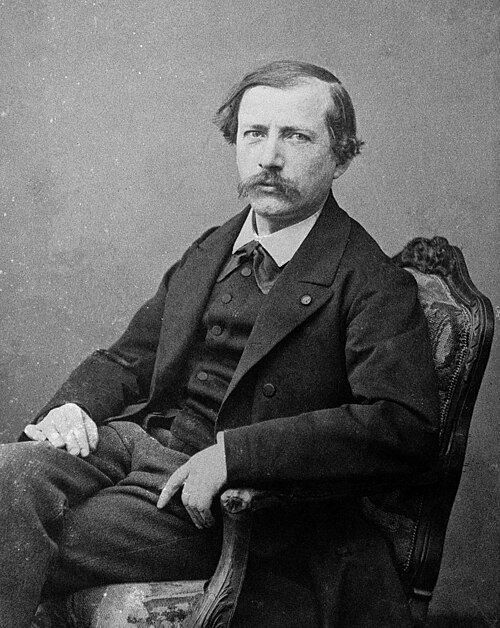
\includegraphics[width=\linewidth]{images/book3/berthelot.jpg}
\end{minipage}\hfill
\begin{minipage}[t]{0.76\linewidth}\vspace{0pt}
马塞兰·贝特洛（1827--1907）用压缩
氧气在内衬铂的密闭钢容器中燃烧有机化合物，使
燃烧完全且无物质逸出：量热弹至今
仍是测定燃烧热的标准仪器。他还创造了
“放热”和“吸热”两词。（照片：公有领域，维基共享资源
）
\end{minipage}
\end{history}

\section{练习}

\begin{exercise}[$\star$]\label{exo:b2:reaction-enthalpy:1}
利用本章的标准摩尔生成焓，计算
丙烷燃烧反应在 \qty{298}{K} 下的 $\Delta_r H^\circ$，
\ce{C3H8(g) + 5O2(g) -> 3CO2(g) + 4H2O(l)}，已知 $\Delta_f
H^\circ(\ce{C3H8}, \text{g}) = \qty{-104.7}{kJ/mol}$。该反应是否
放热？
% ledger: dfh:C3H8_g
\end{exercise}

\begin{exercise}[$\star$]\label{exo:b2:reaction-enthalpy:2}
计算燃烧 \qty{1.00}{kg} 甲烷（生成液态水）及
\qty{1.00}{kg} 氢气所放出的热量，\ce{H2(g) + 1/2O2(g) ->
H2O(l)}。哪种燃料每千克放出的热量更多？
\end{exercise}

\begin{exercise}[$\star$]\label{exo:b2:reaction-enthalpy:3}
弹式量热计给出液态苯燃烧的 $\Delta_r U = \qty{-3264}{kJ/mol}$，
反应式为 \ce{C6H6(l) + 15/2O2(g) -> 6CO2(g) + 3H2O(l)}，温度为
\qty{298}{K}，计算 $\Delta_r H$。
\end{exercise}

\begin{exercise}[$\star$]\label{exo:b2:reaction-enthalpy:4}
已知 $\Delta_r H^\circ = \qty{-393.5}{kJ/mol}$，对应反应 \ce{C(s) + O2(g) ->
CO2(g)}；$\Delta_r H^\circ = \qty{-283.0}{kJ/mol}$，对应反应 \ce{CO(g) +
1/2O2(g) -> CO2(g)}，计算 \ce{CO2(g) + C(s) -> 2CO(g)}
的反应焓，该反应发生在高炉的炽热焦炭中。
\end{exercise}

\begin{exercise}[$\star\star$]\label{exo:b2:reaction-enthalpy:5}
利用本章的键焓估算
\ce{CH4(g) + Cl2(g) -> CH3Cl(g) + HCl(g)}的焓变，取
C--Cl 键焓为 \qty{350}{kJ/mol}。再由生成焓计算同一量，
已知 $\Delta_f H^\circ(\ce{CH3Cl}, \text{g}) = \qty{-83.7}{kJ/mol}$，并
讨论两者的差异。
% ledger: dfh:CH3Cl_g
\end{exercise}

\begin{exercise}[$\star\star$]\label{exo:b2:reaction-enthalpy:6}
水在 \qty{298}{K} 时的标准汽化焓为
$\Delta_f H^\circ(\ce{H2O}, \text{g}) - \Delta_f H^\circ(\ce{H2O},
\text{l})$。计算该值。设液体的 $C_{p,m}^\circ = \qty{75.35}{J/(K.mol)}$，
蒸气的为 \qty{33.59}{J/(K.mol)}，二者均视为
常数，估算 \qty{400}{K} 时的该值（加压下的过热水），
并与数据表比较，数据表给出 $\Delta_f H^\circ =
\qty{-282.59}{kJ/mol}$ 为液体的值，\qty{-242.85}{kJ/mol} 为
蒸气在 \qty{400}{K} 时的值。
% ledger: cp:H2O_l.298, cp:H2O_g.298, janafdfH:H2O_l.400, janafdfH:H2O_g.400
\end{exercise}

\begin{exercise}[$\star\star$]\label{exo:b2:reaction-enthalpy:7}
用玻恩–哈伯循环计算氯化钾的晶格焓，
已知 $\Delta_f H^\circ(\ce{KCl}, \text{s}) = \qty{-436.7}{kJ/mol}$，
钾的升华焓为 \qty{89.0}{kJ/mol}，钾的电离能
为 \qty{4.341}{eV}，$\Delta_f H^\circ(\ce{Cl}, \text{g}) =
\qty{121.3}{kJ/mol}$，氯的电子亲和能为 \qty{3.613}{eV}。
为何氯化钾的晶格焓比氯化钠的小？
% ledger: dfh:KCl_cr, dfh:K_g, ie:K, janaf:Cl, ea:Cl
\end{exercise}

\begin{exercise}[$\star\star$]\label{exo:b2:reaction-enthalpy:8}
以通电方式输入 \qty{2.00}{kJ} 的
电能标定咖啡杯式量热计，使其温度升高 \qty{0.418}{K}。随后
向其中加入 \qty{50.0}{mL} 浓度为 \qty{1.00}{mol/L} 的盐酸，
再与 \qty{50.0}{mL} 浓度为 \qty{1.10}{mol/L} 的氢氧化钠溶液混合，
两者初始温度相同，温度升高
\qty{0.583}{K}。计算下列反应的焓变 \ce{H3O+(aq) + OH-(aq) ->
2H2O(l)}。
\end{exercise}

\begin{exercise}[$\star\star$]\label{exo:b2:reaction-enthalpy:9}
辛烷是汽油的模型物质，其 $\Delta_f H^\circ(\text{l}) =
\qty{-250.3}{kJ/mol}$。计算其燃烧焓（水为液态）、每千克放出的热量，
以及每兆焦所排放的二氧化碳质量，
并与甲烷比较。
% ledger: dfh:C8H18
\end{exercise}

\begin{exercise}[$\star\star\star$]\label{exo:b2:reaction-enthalpy:10}
计算甲烷在化学计量量的纯氧中燃烧的绝热火焰温度，
热容取为常数（即本章 \qty{298}{K} 时的值，
\ce{CO2} 为 37.13，\ce{H2O(g)} 为
\qty{33.59}{J/(K.mol)}）。将其与空气中的结果
（同一近似下为 \qty{2780}{K}）比较。为何纯氧中的真实火焰
远比该计算所示的温度低？
% ledger: cp:CO2_g.298, cp:H2O_g.298
\end{exercise}

\begin{exercise}[$\star\star\star$]\label{exo:b2:reaction-enthalpy:11}
气体的热容常写为 $C_{p,m}^\circ = a + bT$。
对于合成氨反应，取 $\Delta_r a = \qty{-60.5}{J/(K.mol)}$，
$\Delta_r b = \qty{0.0540}{J/(K^2.mol)}$（由数据表在
\qty{300}{K} 与 \qty{800}{K} 之间拟合得到）。应用基尔霍夫定律，自
\qty{298}{K} 积分至 \qty{700}{K}，并与数据表中的值
\qty{-105.2}{kJ/mol}，以及 $C_p$ 为常数时的估算值相比较。
\end{exercise}

\begin{exercise}[$\star\star\star$]\label{exo:b2:reaction-enthalpy:12}
一氧化氮在发动机中由 \ce{N2(g) + O2(g) -> 2NO(g)} 生成。
计算其在 \qty{298}{K} 时的标准反应焓。证明：若
$\Delta_r C_p^\circ$ 较小，则该反应在
\qty{2000}{K} 时吸收的热量与 \qty{298}{K} 时近似相同；利用 \qty{298}{K} 时数据表中的热容，
（\ce{NO} 为 \qty{29.85}{J/(K.mol)}，\ce{N2} 为 29.12，\ce{O2}
为 \qty{29.38}{J/(K.mol)}），估算 \qty{298}{K} 至 \qty{2000}{K} 之间的
变化。解释为何吸热反应可能
恰在最热的火焰中成为问题。
% ledger: dfh:NO_g, cp:NO_g.298, cp:N2_g.298, cp:O2_g.298
\end{exercise}

\section{问题：露营燃气罐}

\begin{problem}[{周末问题——丁烷的能量，一次
弹式量热计中的测量，平底锅中水的加热，以及
火焰的温度}]
\label{pb:b2:reaction-enthalpy:1}
露营炉燃烧的丁烷来自一个装有 \qty{230}{g} 的燃气罐。
\qty{298}{K} 下的数据（$\Delta_f H^\circ$ 的单位为 \unit{kJ/mol}）：\ce{C4H10(g)}
$-125.6$, \ce{CO2(g)} $-393.51$, \ce{H2O(l)} $-285.83$, \ce{H2O(g)}
$-241.83$。摩尔质量：\ce{C4H10} \qty{58.12}{g/mol}，\ce{H2O}
\qty{18.02}{g/mol}。液态水的热容
为 \qty{75.35}{J/(K.mol)}。干空气：\qty{20.95}{\percent} 的 \ce{O2}，
\qty{78.08}{\percent} 的 \ce{N2}，\qty{0.93}{\percent} 的 \ce{Ar}（按体积计）。$R = \qty{8.314}{J/(K.mol)}$。
% ledger: dfh:C4H10_g, dfh:CO2, dfh:H2O-l, dfh:H2O_g, cp:H2O_l.298, air:O2, air:N2, air:Ar

\medskip
\noindent\textbf{第一部分——燃料。}
\begin{enumerate}
  \item 写出丁烷完全燃烧的反应，生成的水为液态，
        按 1 摩尔丁烷计。
  \item 计算其在 \qty{298}{K} 时的标准反应焓。
  \item 若生成的水为蒸气，再计算一次，并解释
        两者之差。
  \item 分别计算两种情形下每克丁烷放出的热量。
  \item 两个数值中，哪一个适用于露营炉，其中的水
        以蒸气形式离开火焰？
  \item 整个燃气罐在炉上能释放多少热量？
\end{enumerate}

\medskip
\noindent\textbf{第二部分——一次测量。}
取 \qty{0.500}{g} 丁烷样品，在弹式量热计中燃烧，该量热计的
热容为 \qty{10.00}{kJ/K}；生成的水凝结。
\begin{enumerate}[resume]
  \item 弹式量热计测量的是什么量？为什么？
  \item 计算第 1 题中反应的 $\Delta\nu_{\text{气体}}$。
  \item 计算预期的 $\Delta_r U$。
  \item 计算量热计的预期温升。
  \item 读得温升为 \qty{2.461}{K}。由此求出测得的 $\Delta_r U$
        及 $\Delta_r H$，并求它们与数据表的相对差。
\end{enumerate}

\medskip
\noindent\textbf{第三部分——水壶。}
\begin{enumerate}[resume]
  \item 计算将 \qty{1.00}{L} 水
        （\qty{1.00}{kg}）从 \qty{20}{\celsius} 加热到 \qty{100}{\celsius} 所需的热量。
  \item 炉具用 \qty{16.0}{g} 丁烷完成此加热。计算其
        效率（水吸收的热量与释放热量之比）。
  \item 其余的热量去了哪里？
  \item 以此效率，整罐燃气能将多少升
        水烧开？
\end{enumerate}

\medskip
\noindent\textbf{第四部分——火焰。}
\begin{enumerate}[resume]
  \item 丁烷在化学计量的空气中燃烧。计算
        每摩尔丁烷所需氧气所伴随的氮气和氩气的
        物质的量。
  \item 列出生成物的物质的量，包括氮气和氩气。
  \item 用两步路径说明，为何该反应在
        \qty{298}{K} 时放出的热量（水为气态）全部用于
        加热这些气体。
  \item 利用 \qty{298}{K} 时的热容：\ce{CO2} 为 37.13，
        \ce{H2O(g)} 为 33.59，\ce{N2} 为 29.12，\ce{Ar} 为 \qty{20.79}{J/(K.mol)}，
        计算生成物的热容。
  \item 在热容视为常数的条件下，求火焰温度。
  \item 数据表给出，每摩尔丁烷的生成物，
        从 \qty{298}{K} 到 \qty{2300}{K} 的焓增为 \qty{2515.7}{kJ}，
        从 \qty{298}{K} 到
        \qty{2400}{K} 的焓增为 \qty{2655.7}{kJ}。用线性插值求火焰温度。
  \item 为什么第一次估算结果偏高？
  \item 丁烷火焰的实测温度为何还要更低？
  \item 写出丁烷在空气中的绝热火焰温度。
\end{enumerate}
\end{problem}
